\documentclass[11pt]{article}

\usepackage[margin=1in]{geometry}
\usepackage[T1]{fontenc}
\usepackage[utf8]{inputenc}
\usepackage{lmodern}
\usepackage{microtype}
\usepackage{amsmath, amssymb}
\usepackage{booktabs}
\usepackage{graphicx}
\usepackage{float}
\usepackage{hyperref}
\usepackage{xcolor}
\usepackage{enumitem}

\hypersetup{
  colorlinks=true,
  linkcolor=blue!60!black,
  citecolor=blue!60!black,
  urlcolor=blue!60!black
}

\setlist[itemize]{leftmargin=*, itemsep=0.35em}
\setlist[enumerate]{leftmargin=*, itemsep=0.35em}

\title{\textbf{DeepLOB on FI-2010 and Optiver}\\\large IEOR 242 Spring 2026 Final Project Report}
\author{Team Information Withheld in Public Repository}
\date{Spring 2026}

\begin{document}
\maketitle

\noindent\textit{This public repository version removes participant identities. Add team names and the presentation link in the private submission copy if needed.}

\begin{abstract}
This project studies whether a deep limit order book model can be both reproduced on a standard benchmark and adapted to a more realistic, shifted market setting. We reproduce DeepLOB on the FI-2010 benchmark using a modern PyTorch pipeline and then transfer the same modeling idea to Optiver auction-book data with only two visible price levels. On FI-2010, we evaluate two training profiles: a paper-style setup that performs best at short horizons and an adaptive, horizon-aware profile that performs best at long horizons. The strongest reproduced FI-2010 result reaches accuracy $0.835$ and MCC $0.608$ at the 10-event horizon, while the adaptive profile reaches MCC $0.694$ at 100 events. We also analyze 104 engineered microstructure factors and show that price/volume derivative features dominate the qualified factor set, while shallow baselines remain well below the deep model. For Optiver, we introduce a transfer pipeline with causal rolling normalization, rolling-quantile labels, and per-stock fine-tuning. The universal zero-shot model reaches mean Cohen's $\kappa = 0.062$ across held-out stocks, and per-stock fine-tuning improves this to $\kappa = 0.084$. The main limitation is that the domain gap remains large: specific-stock out-of-sample training collapses to near-zero agreement, showing that temporal nonstationarity remains a major obstacle.
\end{abstract}

\section{Project Description and Motivation}
The project asks a concrete question: can a high-performing deep architecture for limit order book forecasting be reproduced on a canonical benchmark and then transferred to a materially different market dataset without redesigning the entire model family? We study short-horizon mid-price direction prediction, where the input is a recent sequence of order-book states and the output is a three-class label indicating down, stationary, or up movement over a future horizon.

This is a strong fit for the course because it combines several themes from modern deep learning: structured sequential data, representation learning under distribution shift, model selection under class imbalance, and empirical diagnosis through loss curves and ablations. It is also practically motivated. A model that performs well on a benchmark but fails under a new market representation is still scientifically useful because it reveals where inductive bias transfers and where it breaks.

Our goals are:
\begin{itemize}
  \item reproduce the DeepLOB CNN--Inception--LSTM pipeline on FI-2010 and understand which training configuration is most reliable at each forecast horizon;
  \item test whether the same representation-learning idea transfers to Optiver's shallower two-level auction-book data after architectural adaptation and fine-tuning;
  \item go beyond raw accuracy by comparing against manual-factor baselines and by studying what kinds of microstructure signals appear to drive performance.
\end{itemize}

\section{Data and Learning Problem}
\subsection{Dataset Overview}
We work with two datasets that share the same prediction objective but differ strongly in representation.

\paragraph{FI-2010 benchmark.}
FI-2010 is a standard limit order book benchmark with 40 normalized input features per event, corresponding to 10 bid/ask price levels and their associated volumes. We use the standard three-class mid-price movement task at horizons of 10, 20, 30, 50, and 100 events ahead.

\paragraph{Optiver auction-book data.}
The Optiver workflow uses a two-level book representation derived from processed per-stock files. Each event is represented by 8 reordered features:
\[
\left\{
\begin{array}{l}
\texttt{ask\_price1}, \texttt{ask\_size1}, \texttt{bid\_price1}, \texttt{bid\_size1}, \\
\texttt{ask\_price2}, \texttt{ask\_size2}, \texttt{bid\_price2}, \texttt{bid\_size2}
\end{array}
\right\}.
\]
All reported Optiver experiments use the 5-event prediction horizon and evaluate transfer on held-out stocks 42, 17, and 82.

\paragraph{Sample construction.}
Both workflows convert raw event streams into overlapping windows. For FI-2010, the lookback window is 100 events. For Optiver, the processed stock files are split chronologically into training, validation, and held-out evaluation segments. The exact number of windows depends on horizon and stock, but the learning problem is consistent across both datasets: infer short-horizon direction from recent microstructure state.

\subsection{Learning Task Definition}
Let $X_t \in \mathbb{R}^{100 \times d}$ denote a lookback window ending at event $t$, where $d=40$ for FI-2010 and $d=8$ for Optiver. Let $Y_t \in \{-1,0,+1\}$ denote the future mid-price direction over a horizon of $k$ events. We learn a mapping
\[
f_{\theta}: X_t \mapsto Y_t
\]
that predicts the three-class direction label from the recent order-book trajectory.

For FI-2010 the labels follow the standard benchmark definition. For Optiver, labels are built from future log mid-price returns using rolling quantiles of absolute returns, which makes the class boundaries adapt to the recent volatility scale of each stock.

\subsection{Data Preparation and Quality Considerations}
The main data-quality and preprocessing issues are part of the project itself.

\begin{itemize}
  \item \textbf{Causal preprocessing.} Optiver inputs use causal rolling normalization so each event is standardized using only past observations. This avoids lookahead leakage.
  \item \textbf{Chronological splits.} Both datasets are evaluated with time-aware splits rather than random mixing, because random shuffling would overstate generalization in a time-series setting.
  \item \textbf{Class imbalance.} Short-horizon labels are often dominated by the stationary class. This makes metric choice and checkpointing strategy important.
  \item \textbf{Representation mismatch.} FI-2010 contains 10 visible levels, while Optiver exposes only two. The transfer problem is therefore not just cross-dataset generalization but cross-representation generalization.
  \item \textbf{Nonstationarity.} Within-stock temporal drift on Optiver is severe enough that a model trained on an early window of the same stock can fail on a later window.
\end{itemize}

\section{Methodology}
\subsection{Model Architecture}
\paragraph{DeepLOB on FI-2010.}
Our FI-2010 model follows the DeepLOB architecture closely. The input tensor has shape $(B,1,T,40)$ with $T=100$. The network contains three convolutional blocks that compress local price-volume patterns, an Inception-style module that captures multi-scale local structure, a one-layer LSTM with hidden size 64 that aggregates temporal information, and a dropout plus fully connected classification head. ReLU is used in the hidden layers, and the final three-class prediction is interpreted through a Softmax distribution over logits.

\paragraph{DeepLOBLite on Optiver.}
For Optiver, we adapt the input interface to the shallower book. The model consumes $(B,1,T,8)$ and changes the third convolutional block to use a $(1,2)$ kernel so the network can still aggregate across the narrower spatial dimension. The recurrent and classification components remain largely the same. This produces a lightweight transfer variant we refer to as DeepLOBLite.

\subsection{Objective Function and Training}
We train parameters $\theta$ by solving
\[
\min_{\theta} \frac{1}{N} \sum_{i=1}^{N} L\bigl(f_{\theta}(X_i), Y_i\bigr) + R(\theta).
\]

For FI-2010, $L$ is standard multiclass cross-entropy, optimized with Adam. The paper-style profile uses learning rate $10^{-3}$, batch size 32, and validation-accuracy checkpointing across all five horizons. The adaptive profile changes both regularization and monitoring by horizon, using stronger regularization and validation-loss monitoring at long horizons where overfitting appears earlier.

For Optiver, we use focal loss to mitigate imbalance, dropout of 0.30, weight decay $10^{-4}$, gradient clipping at 1.0, and macro-F1-based model selection. The implementation also includes an auxiliary log-return regression head as a representation regularizer, which stabilizes training under the smaller two-level input representation.

Regularization terms $R(\theta)$ include dropout, $L_2$-style weight decay, early stopping, and in the FI adaptive setting, mild label smoothing and horizon-specific checkpointing. These choices were driven by the empirical failure mode we observed first: naive training often collapsed toward the majority stationary class at short horizons or overfit too early at long horizons.

\subsection{Advanced Component Beyond Class Material}
The main advanced methodological component is the Optiver transfer protocol, which goes beyond simply swapping datasets.

\begin{enumerate}
  \item We construct \textbf{rolling-quantile labels} using the rolling 33rd and 67th percentiles of absolute future returns over a 20{,}000-sample window. This lets the class boundaries adapt to the recent return scale of each stock.
  \item We train a \textbf{universal base model} on source stocks and evaluate it zero-shot on held-out stocks.
  \item We perform \textbf{per-stock fine-tuning} on each held-out stock to recalibrate the classifier to that stock's local return distribution.
\end{enumerate}

This is beyond the lecture baseline because the improvement comes not from making the network deeper, but from explicitly coupling label construction and transfer learning to the target distribution. In practice, this turns out to be more important than adding capacity.

We also add a second advanced element on FI-2010: \textbf{horizon-aware training control}. Instead of using a single checkpointing metric everywhere, the adaptive profile changes its monitor and regularization by horizon. This is a practical but nontrivial design choice that materially improves long-horizon agreement metrics.

\subsection{Baselines and Comparisons}
We compare against baselines that test whether the deep architecture is truly adding value.

\begin{itemize}
  \item On FI-2010, we train ridge logistic regression and a two-layer MLP on 104 engineered microstructure factors.
  \item On Optiver, we compare three regimes: universal zero-shot transfer, per-stock fine-tuning, and specific-stock out-of-sample training.
  \item Across both datasets, we compare the paper-style and adaptive FI training profiles to isolate the effect of training control rather than architecture alone.
\end{itemize}

\section{Experimental Setup}
All experiments were run in a cluster-oriented workflow on PSC Bridges-2 using PyTorch. Heavy training was executed through SLURM jobs, while notebooks were used only to present saved artifacts and diagnostics.

\begin{itemize}
  \item \textbf{Hardware/runtime.} GPU jobs are launched by shell wrappers, and long runs are saved as checkpoints and result files under \texttt{models/} and \texttt{results/}.
  \item \textbf{Software.} The project uses PyTorch, NumPy, pandas, matplotlib, scikit-learn, SciPy, statsmodels, and tqdm.
  \item \textbf{Model selection.} Hyperparameters were tuned through validation performance rather than test feedback. The main comparison is between a paper-faithful FI profile and an adaptive horizon-aware profile, plus several transfer regimes on Optiver.
  \item \textbf{Primary metrics.} We report accuracy, Cohen's $\kappa$, and MCC. These are more informative than raw accuracy alone because the label distribution is often skewed.
  \item \textbf{Secondary diagnostics.} We inspect training/validation loss curves, confusion matrices, baseline comparisons, factor significance plots, and simple proxy profit diagnostics.
\end{itemize}

\section{Results and Discussion}
\subsection{Main Results}
Table~\ref{tab:fi-primary} reports the FI-2010 headline results using the best training profile for each horizon group.

\begin{table}[H]
\centering
\caption{Primary FI-2010 results, using the paper profile for 10--30 events and the adaptive profile for 50--100 events.}
\label{tab:fi-primary}
\begin{tabular}{lcccc}
\toprule
Horizon & Selected profile & Accuracy & $\kappa$ & MCC \\
\midrule
10 events & Paper & 0.8347 & 0.5907 & 0.6080 \\
20 events & Paper & 0.7506 & 0.4879 & 0.5060 \\
30 events & Paper & 0.7726 & 0.5980 & 0.6023 \\
50 events & Adaptive & 0.7940 & 0.6748 & 0.6751 \\
100 events & Adaptive & 0.7944 & 0.6920 & 0.6943 \\
\bottomrule
\end{tabular}
\end{table}

Two patterns matter most. First, the paper-style profile is clearly stronger at short horizons, where validation-accuracy checkpointing prevents the model from drifting too far toward the stationary class. Second, the adaptive profile is slightly but consistently better at 50 and 100 events, where stronger regularization reduces late-stage overfitting.

The factor-analysis and baseline stage supports the same story. Out of 104 engineered microstructure features, 21 survive the full qualification pipeline, and 20 of those belong to the price-and-volume-derivative group. Ridge logistic regression reaches only accuracy $0.710$ with near-zero $\kappa$, while a two-layer MLP improves to MCC $0.191$. DeepLOB reaches accuracy $0.835$ and MCC $0.608$ at the same 10-event horizon, showing that sequence modeling and multi-level feature fusion add far more than a static factor snapshot.

Table~\ref{tab:optiver-main} summarizes the Optiver transfer results.

\begin{table}[H]
\centering
\caption{Optiver 5-event horizon results under rolling-quantile labels, averaged across held-out stocks 42, 17, and 82.}
\label{tab:optiver-main}
\begin{tabular}{lccc}
\toprule
Regime & Mean accuracy & Mean $\kappa$ & Mean MCC \\
\midrule
Universal zero-shot & 0.4211 & 0.0618 & 0.0626 \\
Per-stock fine-tuned & 0.4110 & \textbf{0.0844} & \textbf{0.0847} \\
Specific-stock OOS & 0.3700 & 0.0021 & 0.0021 \\
\bottomrule
\end{tabular}
\end{table}

The Optiver result is conceptually different from the FI benchmark result. Fine-tuning does not raise raw accuracy very much, but it improves $\kappa$ substantially by redistributing predictions away from the dominant class and toward better class agreement. The fact that specific-stock out-of-sample training collapses to near-zero $\kappa$ shows that temporal drift within a stock is at least as difficult as cross-stock transfer.

\subsection{Training and Validation Curves}
\begin{figure}[H]
\centering
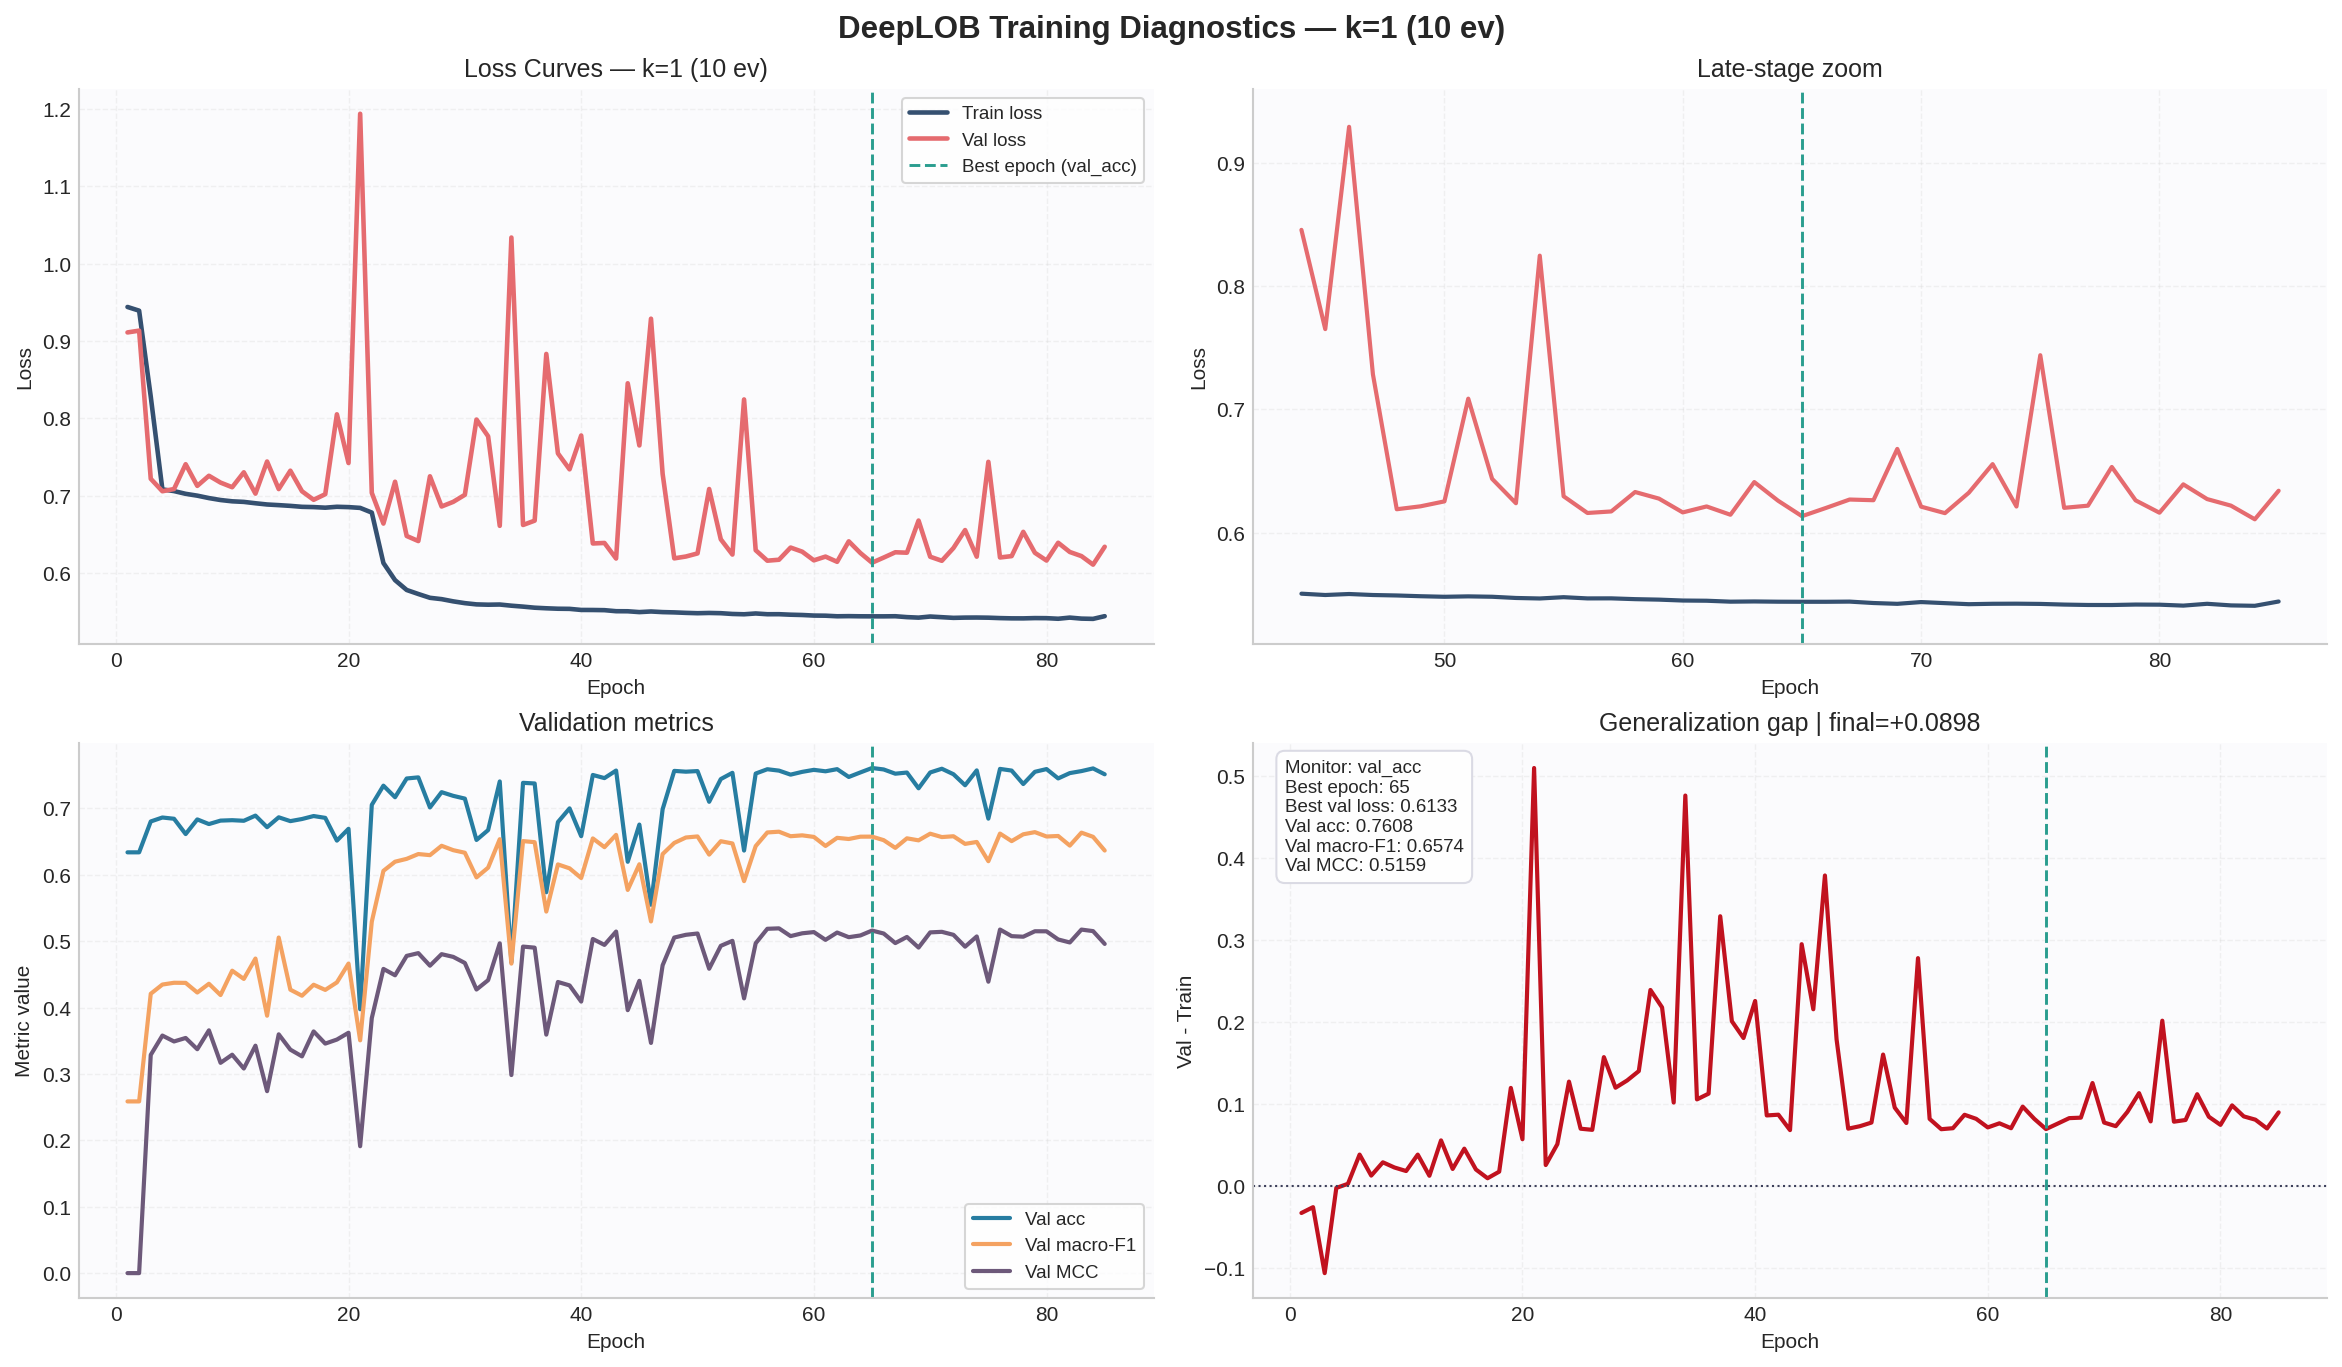
\includegraphics[width=0.72\textwidth]{../results/fi_paper/loss_k0.png}
\caption{FI-2010 training and validation loss at the 10-event horizon under the paper profile. The curve settles after an initially noisy phase, indicating that the model is not simply underfit; the main risk at this horizon is class-collapse under the wrong checkpointing rule rather than inability to optimize.}
\label{fig:fi-loss-k0}
\end{figure}

\begin{figure}[H]
\centering
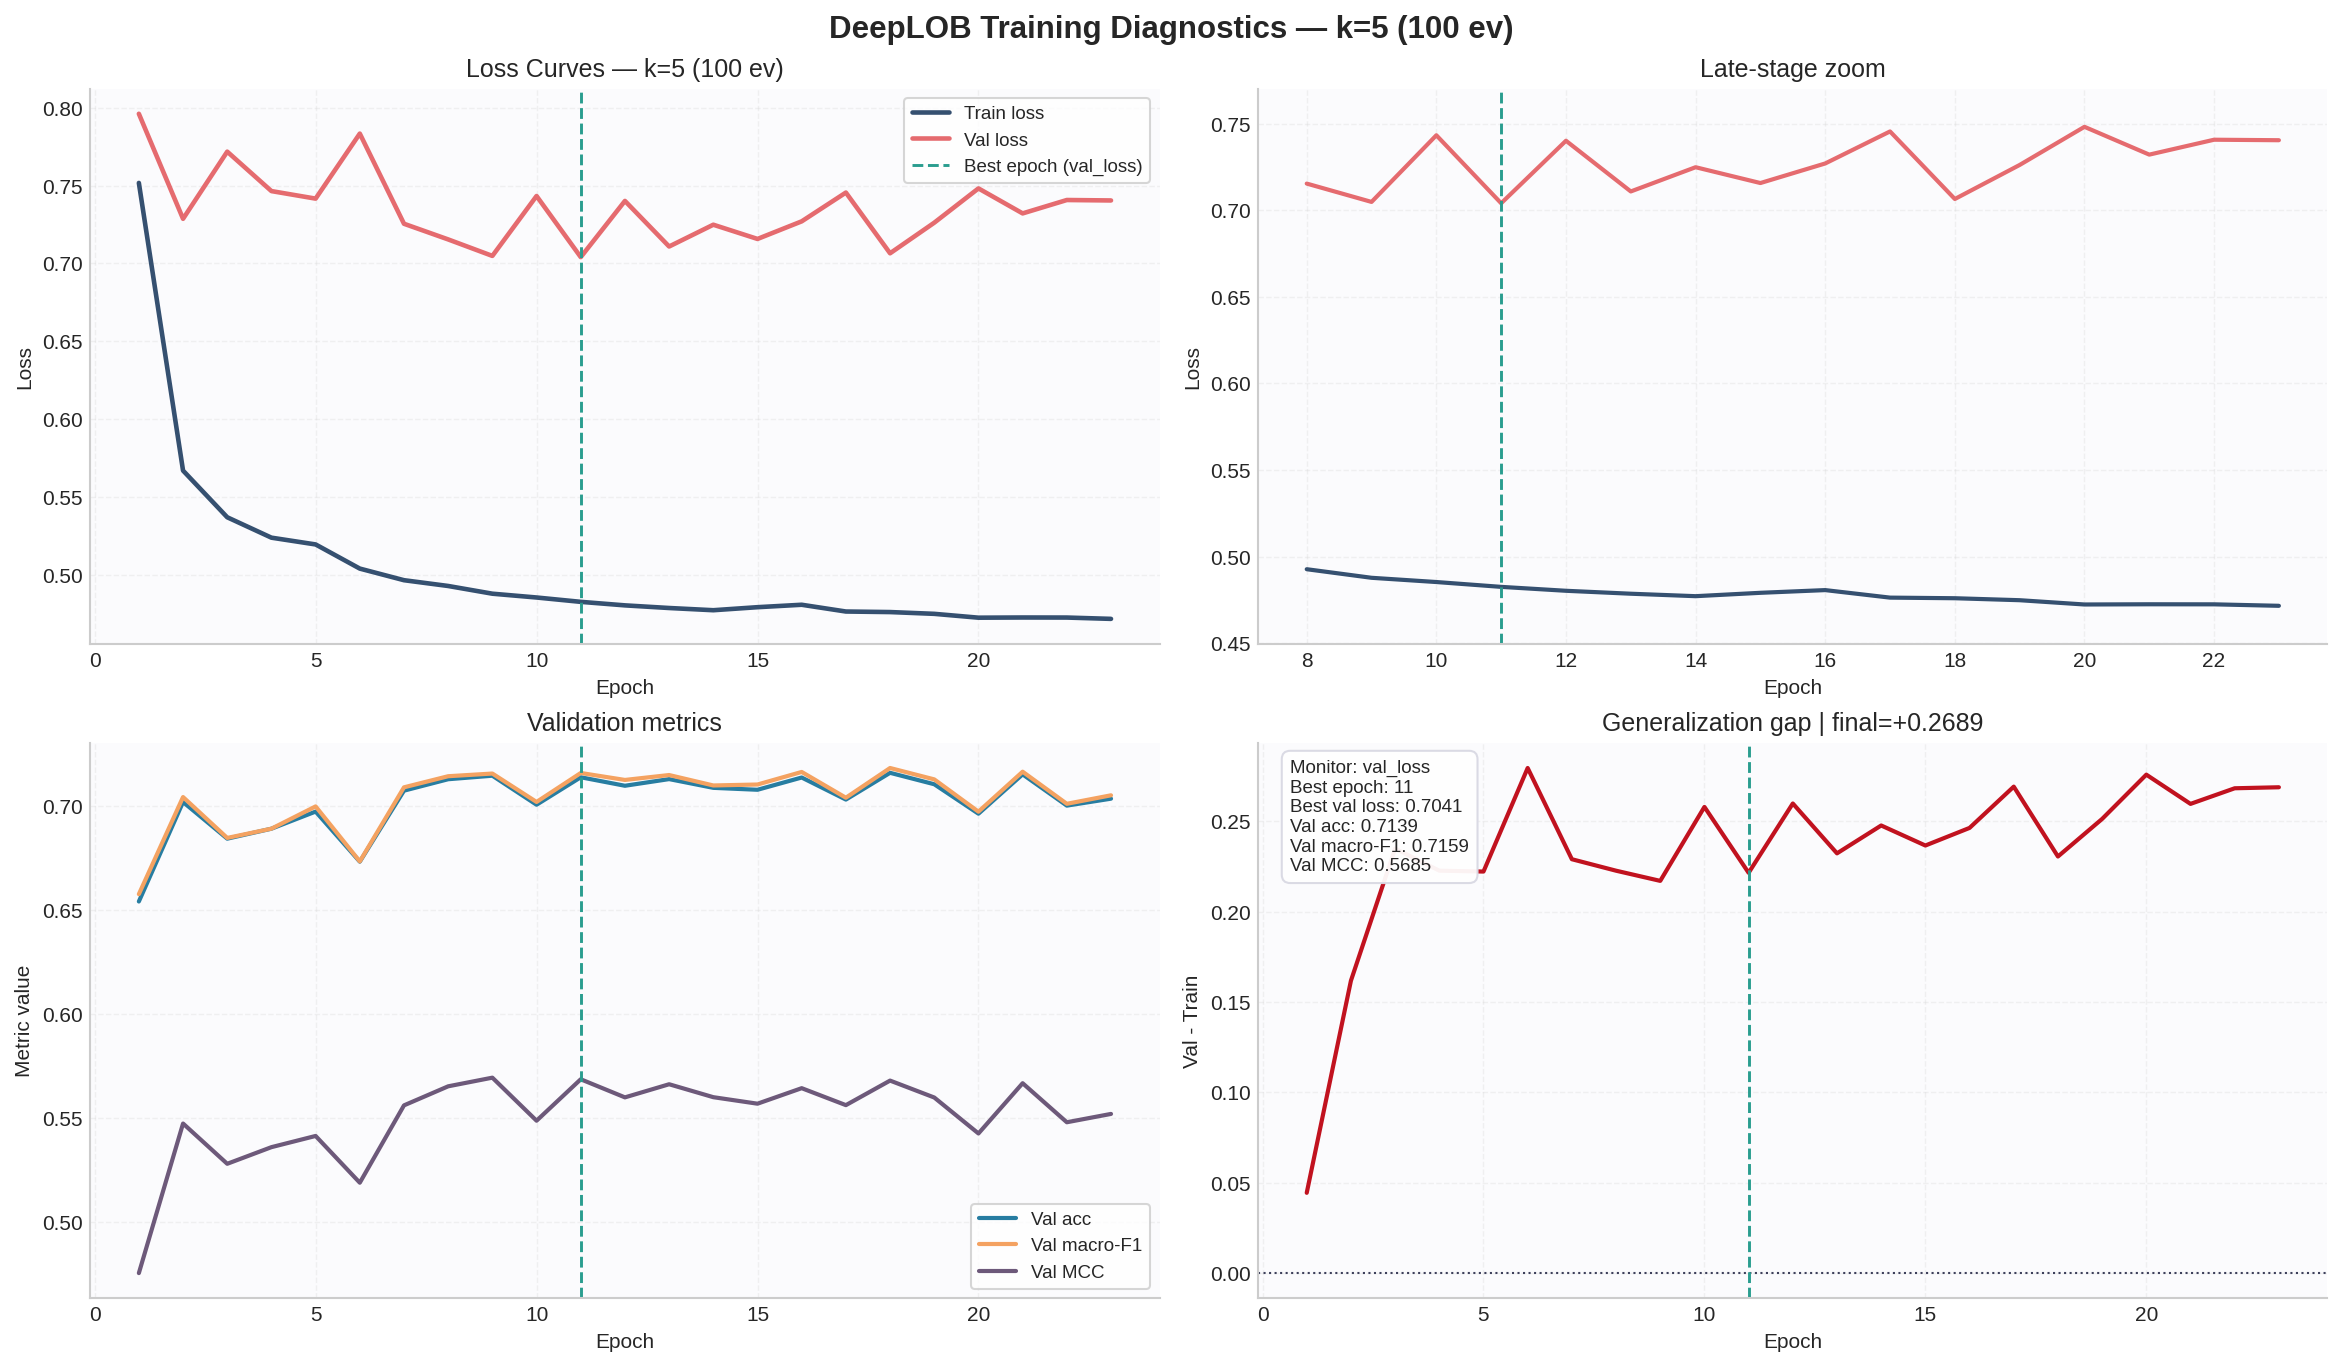
\includegraphics[width=0.72\textwidth]{../results/fi_adaptive/loss_k4.png}
\caption{FI-2010 training and validation loss at the 100-event horizon under the adaptive profile. Compared with the paper-style setting, the adaptive run stops earlier and keeps the validation curve flatter, which is consistent with the long-horizon gain in $\kappa$ and MCC.}
\label{fig:fi-loss-k4}
\end{figure}

\begin{figure}[H]
\centering
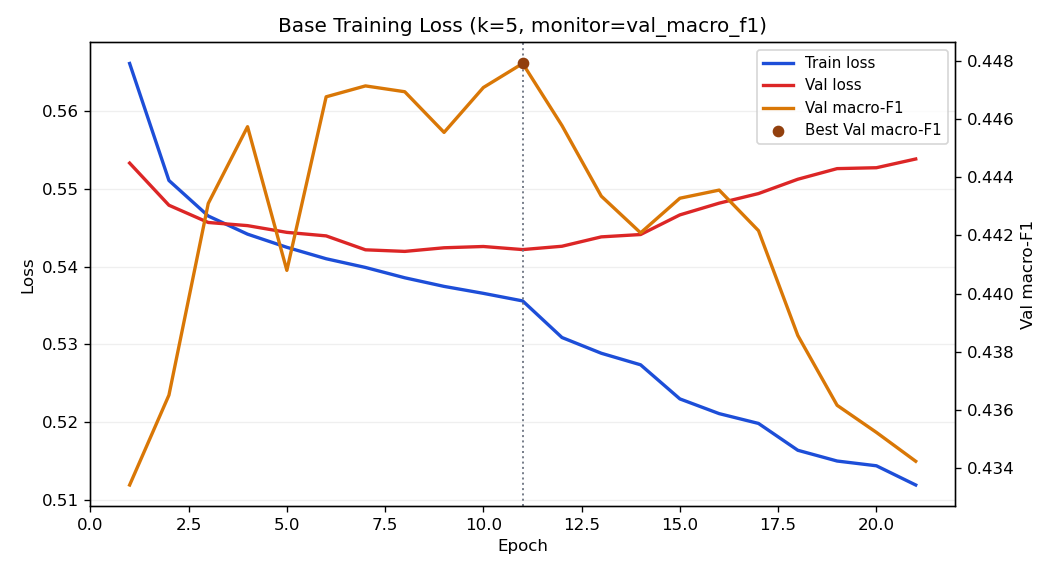
\includegraphics[width=0.72\textwidth]{../results/optiver/classification_rolling3_w20000/base_loss_k5.png}
\caption{Optiver universal base-model loss curve for the 5-event horizon. Optimization is stable, so the bottleneck on Optiver is not obvious divergence; it is the mismatch between the learned representation and the held-out stock distribution.}
\label{fig:optiver-loss}
\end{figure}

\subsection{Interpretation}
The loss curves help diagnose where the project succeeds and where it still falls short. On FI-2010, the short-horizon model is not obviously underfit. Instead, the critical issue is whether training control preserves minority-class predictive power. At long horizons, the gap between the paper and adaptive profiles is more consistent with mild overfitting, which is why stronger regularization helps.

On Optiver, the losses converge cleanly, but clean optimization does not translate into strong generalization. That is exactly the point of the transfer experiment: the architecture can fit the training data, yet still struggle because the book depth, label construction, and local return scales differ across stocks. Per-stock fine-tuning helps because it recalibrates the classifier to the target stock. However, the absolute performance level remains modest, so this is not a production-ready trading model.

The best scientific takeaway is therefore not ``DeepLOB solves the whole problem.'' It is more specific: the architecture is genuinely strong on the standard benchmark, and some of its representation transfers to Optiver, but label adaptation and stock-specific recalibration matter more than simply reusing the pretrained model unchanged.

\begin{figure}[H]
\centering
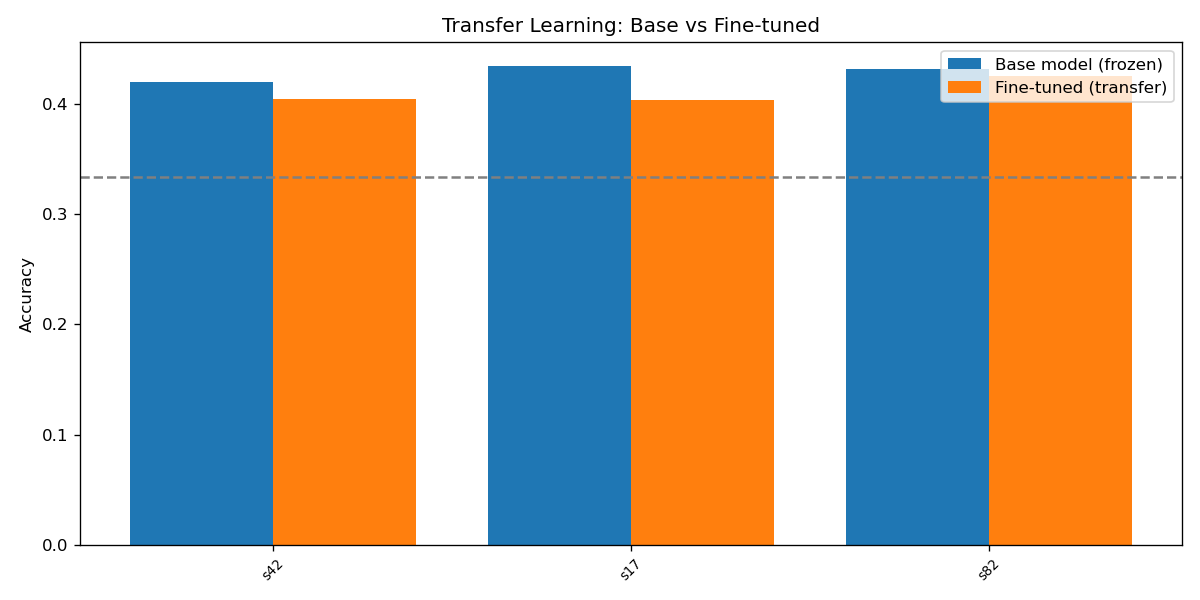
\includegraphics[width=0.72\textwidth]{../results/optiver/classification_rolling3_w20000/transfer_comparison_k5.png}
\caption{Comparison of Optiver evaluation regimes. Fine-tuning consistently improves agreement over zero-shot transfer, while specific-stock out-of-sample training collapses, highlighting temporal nonstationarity as the main remaining failure mode.}
\label{fig:optiver-transfer}
\end{figure}

\section{Safety, Security, and Ethics}
If a model like this were deployed at scale, the main concern would not be benchmark accuracy but how errors interact with a live financial system. A model that overpredicts short-term direction could amplify trading volume, create unstable feedback loops, or encourage users to trust patterns that disappear after regime shifts. This risk is particularly serious here because the Optiver experiments show strong nonstationarity: a model that looks calibrated on one period can fail badly on another.

Security is also relevant. Market data pipelines are vulnerable to silent leakage, preprocessing mistakes, and distribution shifts that are not obvious from a single aggregate metric. A malicious or low-quality data source could effectively poison the learned decision boundary. Because this project uses rolling normalization and rolling-quantile labels, incorrect temporal ordering or accidental lookahead would produce misleadingly strong results. That makes auditability and reproducibility important technical safeguards, not just good style.

There are also ethical and institutional issues. Access to fast market data and large compute budgets is uneven, so automated trading models can reinforce existing inequalities in who can participate effectively. If a model were marketed as decision support without clear uncertainty communication, less sophisticated users could be exposed to disproportionate risk. The current results are therefore better interpreted as research diagnostics than as a basis for autonomous trading.

Reasonable mitigations would include conservative deployment thresholds, abstention near the decision boundary, strict chronological validation, post-deployment drift monitoring, and human oversight. Given the present Optiver transfer performance, the appropriate conclusion is that the model should not be deployed without substantial additional calibration and risk controls.

\section{Presentation Summary}
The recorded presentation for this project should emphasize the following flow:

\begin{enumerate}
  \item motivate short-horizon limit order book prediction as a structured deep learning problem;
  \item explain the difference between the FI-2010 benchmark and the Optiver transfer setting;
  \item walk through the DeepLOB and DeepLOBLite architectures, the objective function, and the advanced transfer methodology;
  \item present the FI benchmark results, loss-curve diagnostics, baseline comparison, and Optiver transfer table;
  \item close with the main limitation: benchmark success transfers only partially because temporal nonstationarity remains severe.
\end{enumerate}

In the private submission copy, this section can also include the team members and the recording link.

\section{Conclusion}
This project turned a generic deep learning assignment prompt into a concrete empirical study of reproduction and transfer. On FI-2010, DeepLOB reproduces strongly, with the paper-style profile working best at short horizons and the adaptive profile working best at long horizons. On Optiver, the architecture still extracts useful signal, but the best gains come from rolling-quantile labels and per-stock fine-tuning rather than naive zero-shot reuse.

The strongest conclusion is that architecture alone is not the full story. For real financial sequence data, label design, calibration, and evaluation protocol matter as much as the neural backbone. That makes this project a useful example of how deep learning methodology has to be adapted carefully to the structure of the application domain rather than applied as a plug-and-play recipe.

\end{document}